\documentclass{standalone}
\usepackage{tikz}
\usetikzlibrary{patterns, positioning}


\begin{document}
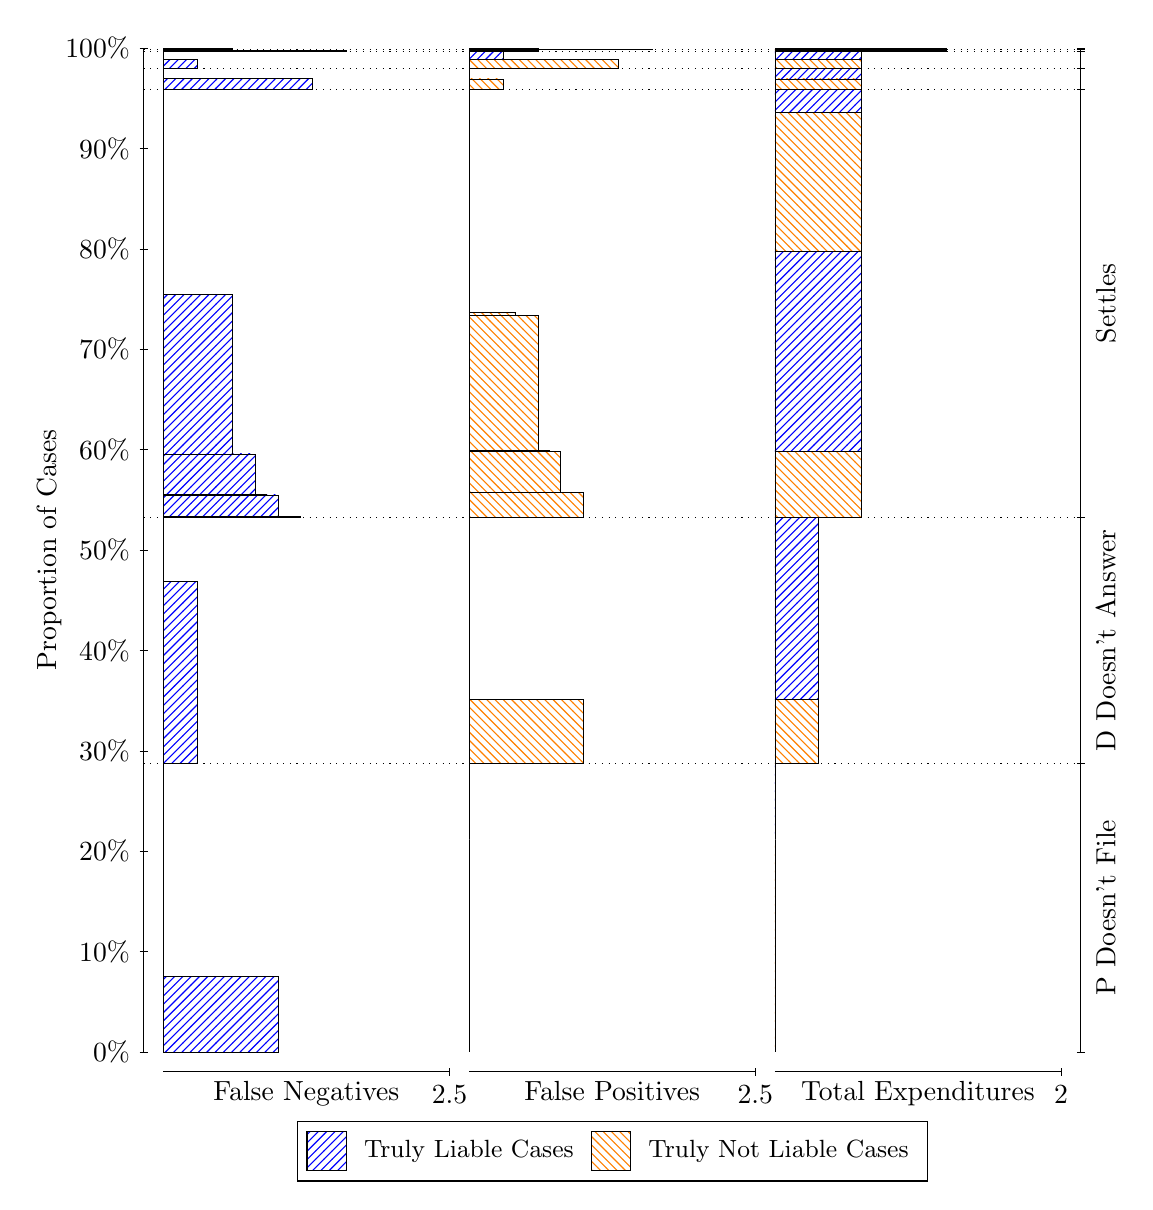
\begin{tikzpicture}
\draw[black, very thin] (1.5,1.75) -- (1.5,14.5);
\node[rotate=90, text=black, anchor=center] at (0.3, 8.125) {Proportion of Cases};
\draw[black, very thin] (1.45,1.75) -- (1.55,1.75);
\node[text=black, anchor=east] at (1.45, 1.75) {0\%};
\draw[black, very thin] (1.45,3.025) -- (1.55,3.025);
\node[text=black, anchor=east] at (1.45, 3.025) {10\%};
\draw[black, very thin] (1.45,4.3) -- (1.55,4.3);
\node[text=black, anchor=east] at (1.45, 4.3) {20\%};
\draw[black, very thin] (1.45,5.575) -- (1.55,5.575);
\node[text=black, anchor=east] at (1.45, 5.575) {30\%};
\draw[black, very thin] (1.45,6.85) -- (1.55,6.85);
\node[text=black, anchor=east] at (1.45, 6.85) {40\%};
\draw[black, very thin] (1.45,8.125) -- (1.55,8.125);
\node[text=black, anchor=east] at (1.45, 8.125) {50\%};
\draw[black, very thin] (1.45,9.4) -- (1.55,9.4);
\node[text=black, anchor=east] at (1.45, 9.4) {60\%};
\draw[black, very thin] (1.45,10.675) -- (1.55,10.675);
\node[text=black, anchor=east] at (1.45, 10.675) {70\%};
\draw[black, very thin] (1.45,11.95) -- (1.55,11.95);
\node[text=black, anchor=east] at (1.45, 11.95) {80\%};
\draw[black, very thin] (1.45,13.225) -- (1.55,13.225);
\node[text=black, anchor=east] at (1.45, 13.225) {90\%};
\draw[black, very thin] (1.45,14.5) -- (1.55,14.5);
\node[text=black, anchor=east] at (1.45, 14.5) {100\%};

\draw[black, very thin] (13.4,1.75) -- (13.4,14.5);
\draw[black, very thin] (13.35,1.75) -- (13.45,1.75);
\node[anchor=west] at (13.35, 1.75) {};
\draw[black, very thin] (13.35,5.4139) -- (13.45,5.4139);
\node[anchor=west] at (13.35, 5.4139) {};
\draw[black, very thin] (13.35,8.5376) -- (13.45,8.5376);
\node[anchor=west] at (13.35, 8.5376) {};
\draw[black, very thin] (13.35,13.978) -- (13.45,13.978);
\node[anchor=west] at (13.35, 13.978) {};
\draw[black, very thin] (13.35,14.243) -- (13.45,14.243);
\node[anchor=west] at (13.35, 14.243) {};
\draw[black, very thin] (13.35,14.46) -- (13.45,14.46);
\node[anchor=west] at (13.35, 14.46) {};
\draw[black, very thin] (13.35,14.48) -- (13.45,14.48);
\node[anchor=west] at (13.35, 14.48) {};
\draw[black, very thin] (13.35,14.5) -- (13.45,14.5);
\node[anchor=west] at (13.35, 14.5) {};

\draw[black, very thin, pattern color=blue, pattern=north east lines] (1.75,1.75) rectangle (3.2033,2.7129);
\draw[black, very thin, pattern color=orange, pattern=north west lines] (1.75,2.7129) rectangle (1.75,5.4139);
\draw[black, very thin, pattern color=blue, pattern=north east lines] (1.75,5.4139) rectangle (2.186,7.7263);
\draw[black, very thin, pattern color=orange, pattern=north west lines] (1.75,7.7263) rectangle (1.75,8.5376);
\draw[black, very thin, pattern color=blue, pattern=north east lines] (1.75,8.5376) rectangle (3.494,8.5473);
\draw[black, very thin, pattern color=blue, pattern=north east lines] (1.75,8.5473) rectangle (3.2033,8.8258);
\draw[black, very thin, pattern color=blue, pattern=north east lines] (1.75,8.8258) rectangle (3.058,8.8329);
\draw[black, very thin, pattern color=blue, pattern=north east lines] (1.75,8.8329) rectangle (2.9127,9.3455);
\draw[black, very thin, pattern color=blue, pattern=north east lines] (1.75,9.3455) rectangle (2.622,11.374);
\draw[black, very thin, pattern color=orange, pattern=north west lines] (1.75,11.374) rectangle (1.75,13.978);
\draw[black, very thin, pattern color=blue, pattern=north east lines] (1.75,13.978) rectangle (3.6393,14.112);
\draw[black, very thin, pattern color=orange, pattern=north west lines] (1.75,14.112) rectangle (1.75,14.243);
\draw[black, very thin, pattern color=blue, pattern=north east lines] (1.75,14.243) rectangle (2.186,14.351);
\draw[black, very thin, pattern color=orange, pattern=north west lines] (1.75,14.351) rectangle (1.75,14.46);
\draw[black, very thin, pattern color=blue, pattern=north east lines] (1.75,14.46) rectangle (4.0753,14.467);
\draw[black, very thin, pattern color=orange, pattern=north west lines] (1.75,14.467) rectangle (1.75,14.48);
\draw[black, very thin, pattern color=blue, pattern=north east lines] (1.75,14.48) rectangle (2.622,14.494);
\draw[black, very thin, pattern color=orange, pattern=north west lines] (1.75,14.494) rectangle (1.75,14.5);
\draw[black, very thin, pattern color=orange, pattern=north west lines] (5.6333,1.75) rectangle (5.6333,4.451);
\draw[black, very thin, pattern color=blue, pattern=north east lines] (5.6333,4.451) rectangle (5.6333,5.4139);
\draw[black, very thin, pattern color=orange, pattern=north west lines] (5.6333,5.4139) rectangle (7.0867,6.2252);
\draw[black, very thin, pattern color=blue, pattern=north east lines] (5.6333,6.2252) rectangle (5.6333,8.5376);
\draw[black, very thin, pattern color=orange, pattern=north west lines] (5.6333,8.5376) rectangle (7.0867,8.8586);
\draw[black, very thin, pattern color=orange, pattern=north west lines] (5.6333,8.8586) rectangle (6.796,9.3794);
\draw[black, very thin, pattern color=orange, pattern=north west lines] (5.6333,9.3794) rectangle (6.6507,9.3935);
\draw[black, very thin, pattern color=orange, pattern=north west lines] (5.6333,9.3935) rectangle (6.5053,11.103);
\draw[black, very thin, pattern color=orange, pattern=north west lines] (5.6333,11.103) rectangle (6.2147,11.141);
\draw[black, very thin, pattern color=blue, pattern=north east lines] (5.6333,11.141) rectangle (5.6333,13.978);
\draw[black, very thin, pattern color=orange, pattern=north west lines] (5.6333,13.978) rectangle (6.0693,14.108);
\draw[black, very thin, pattern color=blue, pattern=north east lines] (5.6333,14.108) rectangle (5.6333,14.243);
\draw[black, very thin, pattern color=orange, pattern=north west lines] (5.6333,14.243) rectangle (7.5227,14.353);
\draw[black, very thin, pattern color=blue, pattern=north east lines] (5.6333,14.353) rectangle (6.0693,14.46);
\draw[black, very thin, pattern color=orange, pattern=north west lines] (5.6333,14.46) rectangle (6.5053,14.473);
\draw[black, very thin, pattern color=blue, pattern=north east lines] (5.6333,14.473) rectangle (5.6333,14.48);
\draw[black, very thin, pattern color=orange, pattern=north west lines] (5.6333,14.48) rectangle (7.9587,14.486);
\draw[black, very thin, pattern color=blue, pattern=north east lines] (5.6333,14.486) rectangle (6.5053,14.5);
\draw[black, very thin, pattern color=orange, pattern=north west lines] (9.5167,1.75) rectangle (9.5167,4.451);
\draw[black, very thin, pattern color=blue, pattern=north east lines] (9.5167,4.451) rectangle (9.5167,5.4139);
\draw[black, very thin, pattern color=orange, pattern=north west lines] (9.5167,5.4139) rectangle (10.062,6.2252);
\draw[black, very thin, pattern color=blue, pattern=north east lines] (9.5167,6.2252) rectangle (10.062,8.5376);
\draw[black, very thin, pattern color=orange, pattern=north west lines] (9.5167,8.5376) rectangle (10.607,9.3794);
\draw[black, very thin, pattern color=blue, pattern=north east lines] (9.5167,9.3794) rectangle (10.607,11.921);
\draw[black, very thin, pattern color=orange, pattern=north west lines] (9.5167,11.921) rectangle (10.607,13.682);
\draw[black, very thin, pattern color=blue, pattern=north east lines] (9.5167,13.682) rectangle (10.607,13.978);
\draw[black, very thin, pattern color=orange, pattern=north west lines] (9.5167,13.978) rectangle (10.607,14.108);
\draw[black, very thin, pattern color=blue, pattern=north east lines] (9.5167,14.108) rectangle (10.607,14.243);
\draw[black, very thin, pattern color=orange, pattern=north west lines] (9.5167,14.243) rectangle (10.607,14.353);
\draw[black, very thin, pattern color=blue, pattern=north east lines] (9.5167,14.353) rectangle (10.607,14.46);
\draw[black, very thin, pattern color=orange, pattern=north west lines] (9.5167,14.46) rectangle (11.697,14.473);
\draw[black, very thin, pattern color=blue, pattern=north east lines] (9.5167,14.473) rectangle (11.697,14.48);
\draw[black, very thin, pattern color=orange, pattern=north west lines] (9.5167,14.48) rectangle (11.697,14.486);
\draw[black, very thin, pattern color=blue, pattern=north east lines] (9.5167,14.486) rectangle (11.697,14.5);
\draw[black, dotted] (1.5,5.4139) -- (13.4,5.4139);
\draw[black, dotted] (1.5,8.5376) -- (13.4,8.5376);
\draw[black, dotted] (1.5,13.978) -- (13.4,13.978);
\draw[black, dotted] (1.5,14.243) -- (13.4,14.243);
\draw[black, dotted] (1.5,14.46) -- (13.4,14.46);
\draw[black, dotted] (1.5,14.48) -- (13.4,14.48);
\draw[black, very thin] (1.75,1.5) -- (5.3833,1.5);
\node[text=black, anchor=north] at (3.5667, 1.5) {False Negatives};
\draw[black, very thin] (5.3833,1.45) -- (5.3833,1.55);
\node[text=black, anchor=north] at (5.3833, 1.45) {2.5};

\draw[black, very thin] (5.6333,1.5) -- (9.2667,1.5);
\node[text=black, anchor=north] at (7.45, 1.5) {False Positives};
\draw[black, very thin] (9.2667,1.45) -- (9.2667,1.55);
\node[text=black, anchor=north] at (9.2667, 1.45) {2.5};

\draw[black, very thin] (9.5167,1.5) -- (13.15,1.5);
\node[text=black, anchor=north] at (11.333, 1.5) {Total Expenditures};
\draw[black, very thin] (13.15,1.45) -- (13.15,1.55);
\node[text=black, anchor=north] at (13.15, 1.45) {2};

\node[text=black, centered, rotate=90] at (13.72, 3.5819) {P Doesn't File};
\node[text=black, centered, rotate=90] at (13.72, 6.9758) {D Doesn't Answer};
\node[text=black, centered, rotate=90] at (13.72, 11.258) {Settles};





\draw (7.449999999999999,1.5) node[draw=none] (baseCoordinate) {};
\begin{scope}[align=center]
        \matrix[scale=0.5, draw=black, below=0.5cm of baseCoordinate, nodes={draw}, column sep=0.1cm]{
            \node[rectangle, draw, minimum width=0.5cm, minimum height=0.5cm, pattern color=blue, pattern=north east lines] {}; &
            \node[draw=none, font=\small, text=black] (B) {Truly Liable Cases}; &
            \node[rectangle, draw, minimum width=0.5cm, minimum height=0.5cm, pattern color=orange, pattern=north west lines] {}; &
            \node[draw=none, font=\small, text=black] (B) {Truly Not Liable Cases}; \\
            };
\end{scope}

\end{tikzpicture}
\end{document}